\documentclass{rapport}
\usepackage{pythontex}
\usepackage{csquotes}
\addbibresource{library.bib}


\begin{document}

%----------- Informations du rapport ---------

\unif{HEIG-VD}
\titre{Titre} %Titre du fichier .pdf
\cours{Cours} %Nom du cours
\sujet{Sujet} %Nom du sujet
\groupe{Groupe} %Nom du groupe

\enseignant{Bruce  \textsc{Wayne} \\
            Tony  \textsc{Stark}} %Nom de l'enseignant

\eleves{James   \textsc{Bond} \\
        James  \textsc{Bond}\\
        James \textsc{Bond}} %Nom des élèves

\nom{James Bond, James Bond, James Bond} %nom dans l'entête

%----------- Initialisation -------------------


\fairepagedegarde %Créer la page de garde
\thispagestyle{noPage}
\tabledematieres %Créer la table de matières
\thispagestyle{noPage}
\newpage
\listoffigures
\listoftables
\clearpage
\setcounter{page}{1}
\fairemarges %Afficher les marges
%------------ Corps du rapport ----------------


\input{Chapitres/ch1Py.tex}

\section{Introduction}


\subsection{But}



    


\input{Chapitres/ch2Py.tex}

\section{Joint SF}

\subsection{Fonctionnement du système}


\input{Chapitres/ch3Py.tex}

\section{Cylindre}

\subsection{Fonctionnement du système}

\input{Chapitres/ch4Py.tex}

\section{Préhenseur}

\subsection{Fonctionnement du système}
\subsubsection{Préhenseur}


\input{Chapitres/ch5.tex}
%%------------- Commandes utiles ----------------

\section{Quelques commandes}

Voici quelques commandes utiles :

%------ Pour insérer et citer une image centralisée -----

\insererfigure{logos/Import.jpg}{3cm}{Légende de la figure}{Label de la figure}
% Le premier argument est le chemin pour la photo
% Le deuxième est la hauteur de la photo
% Le troisième la légende
% Le quatrième le label
Ici, je cite l'image \ref{fig: Label de la figure}


%------- Pour insérer et citer une équation --------------

\begin{equation} \label{eq: exemple}
\rho + \Delta = 42
\end{equation}

L'équation \ref{eq: exemple} est cité ici. 

% ------- Pour écrire des variables ----------------------

Pour écrire des variables dans le texte, il suffit de mettre le symbole \$ entre le texte souhaité comme : constante $\rho$.

Pour utiliser pythontex : (pour les chapitres un fichier tex séparé pour python a été préparé)
\begin{pycode}
x = 3
\end{pycode}
       
$x = \py{x}$

si x = ?? effectuer :
pythontex main.tex


Pour créer une bibliography avec des citations :

Ceci est du texte avec une citation complète comme note de bas de page.\footfullcite{smith2023}
Ceci est un référence d'un site \footfullcite{Biscactus}
Ceci est un référence d'un site \footfullcite{LaTeX}

\begin{table}[H]
    \centering
    \textbf{Titre}

    \vspace{0.3cm}
    \begin{tabular}{|l|l|}
    \hline
    Avantages & Inconvénients \\ \hline
      robuste        &   système déséquilibré  \\ \hline
       coût d'usinage réduit       &     \\ \hline
    \end{tabular}
    \caption{Avantages, inconvénients conception générale 3}
    \label{tab:idGen3}
    \end{table}



\begin{flushright}
    Yverdon, {\today\par}
\end{flushright}
% \vspace{1cm}

\begin{figure}[H]
    \centering
    \begin{minipage}[b]{0.3\textwidth}
      \centering
      James Bond\\
      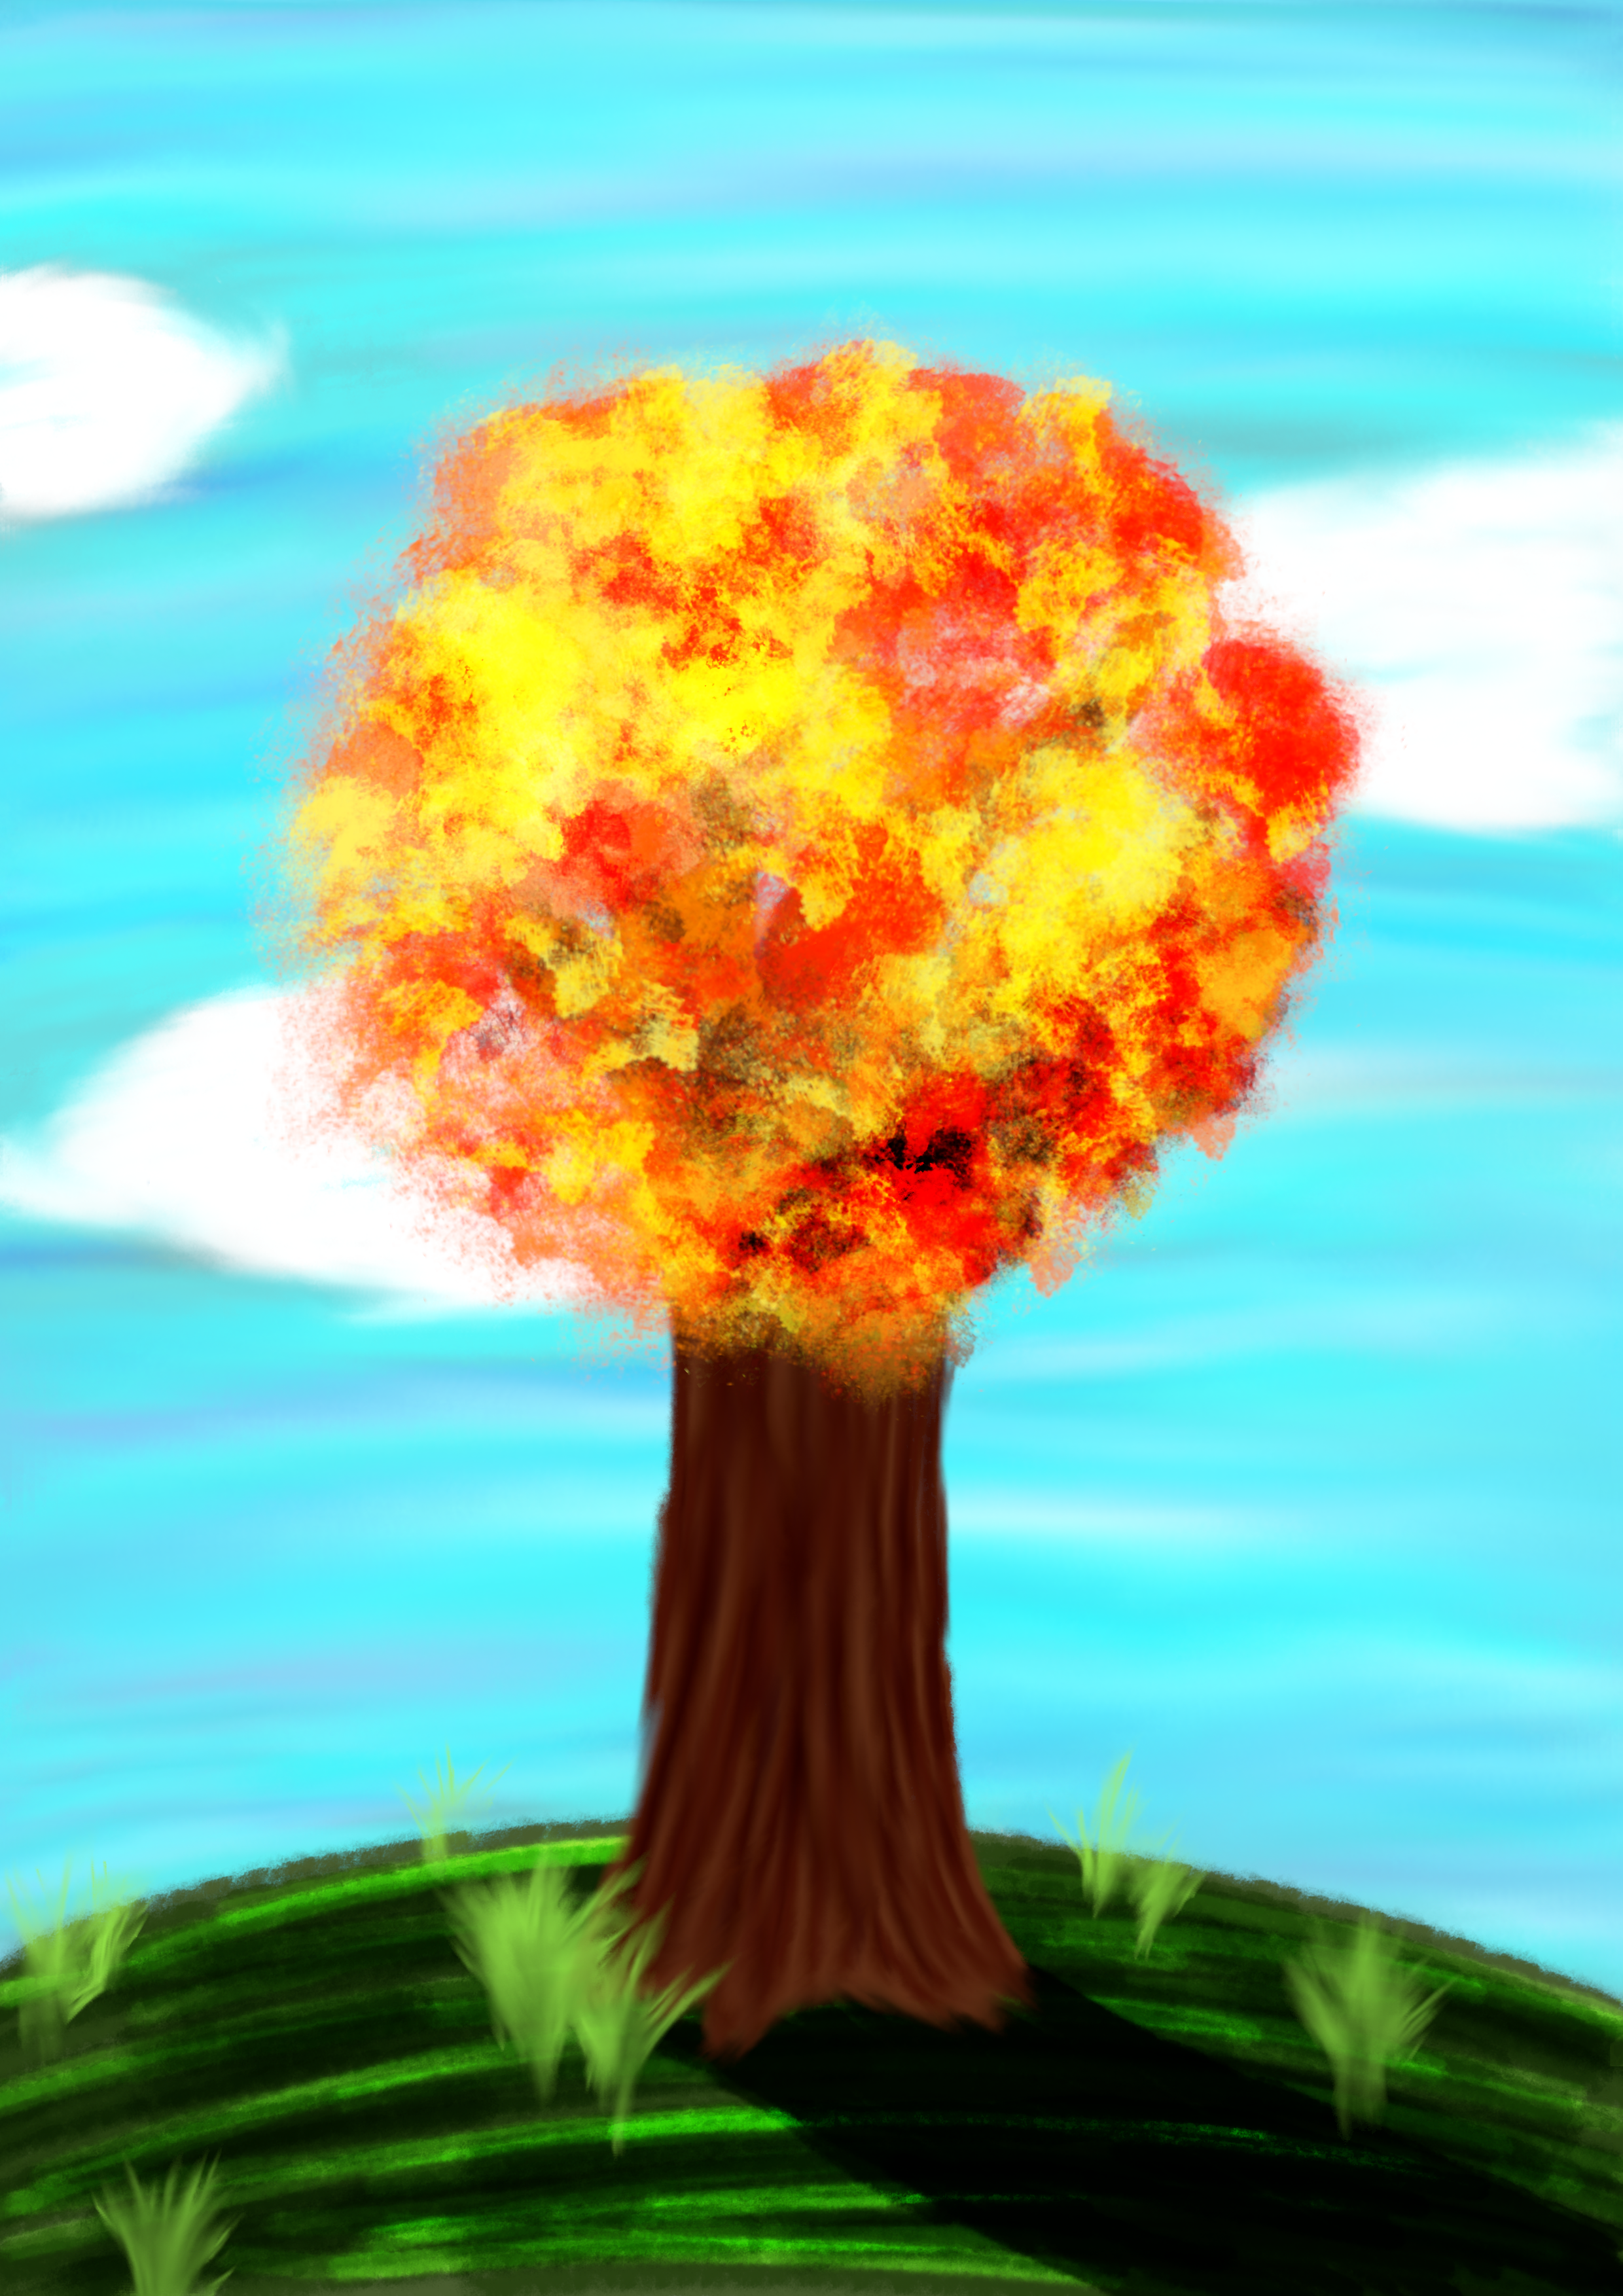
\includegraphics[height=0.4\textwidth]{logos/arbre.png}
    \end{minipage}
    \hfill
    \begin{minipage}[b]{0.3\textwidth}
      \centering
      James Bond\\
      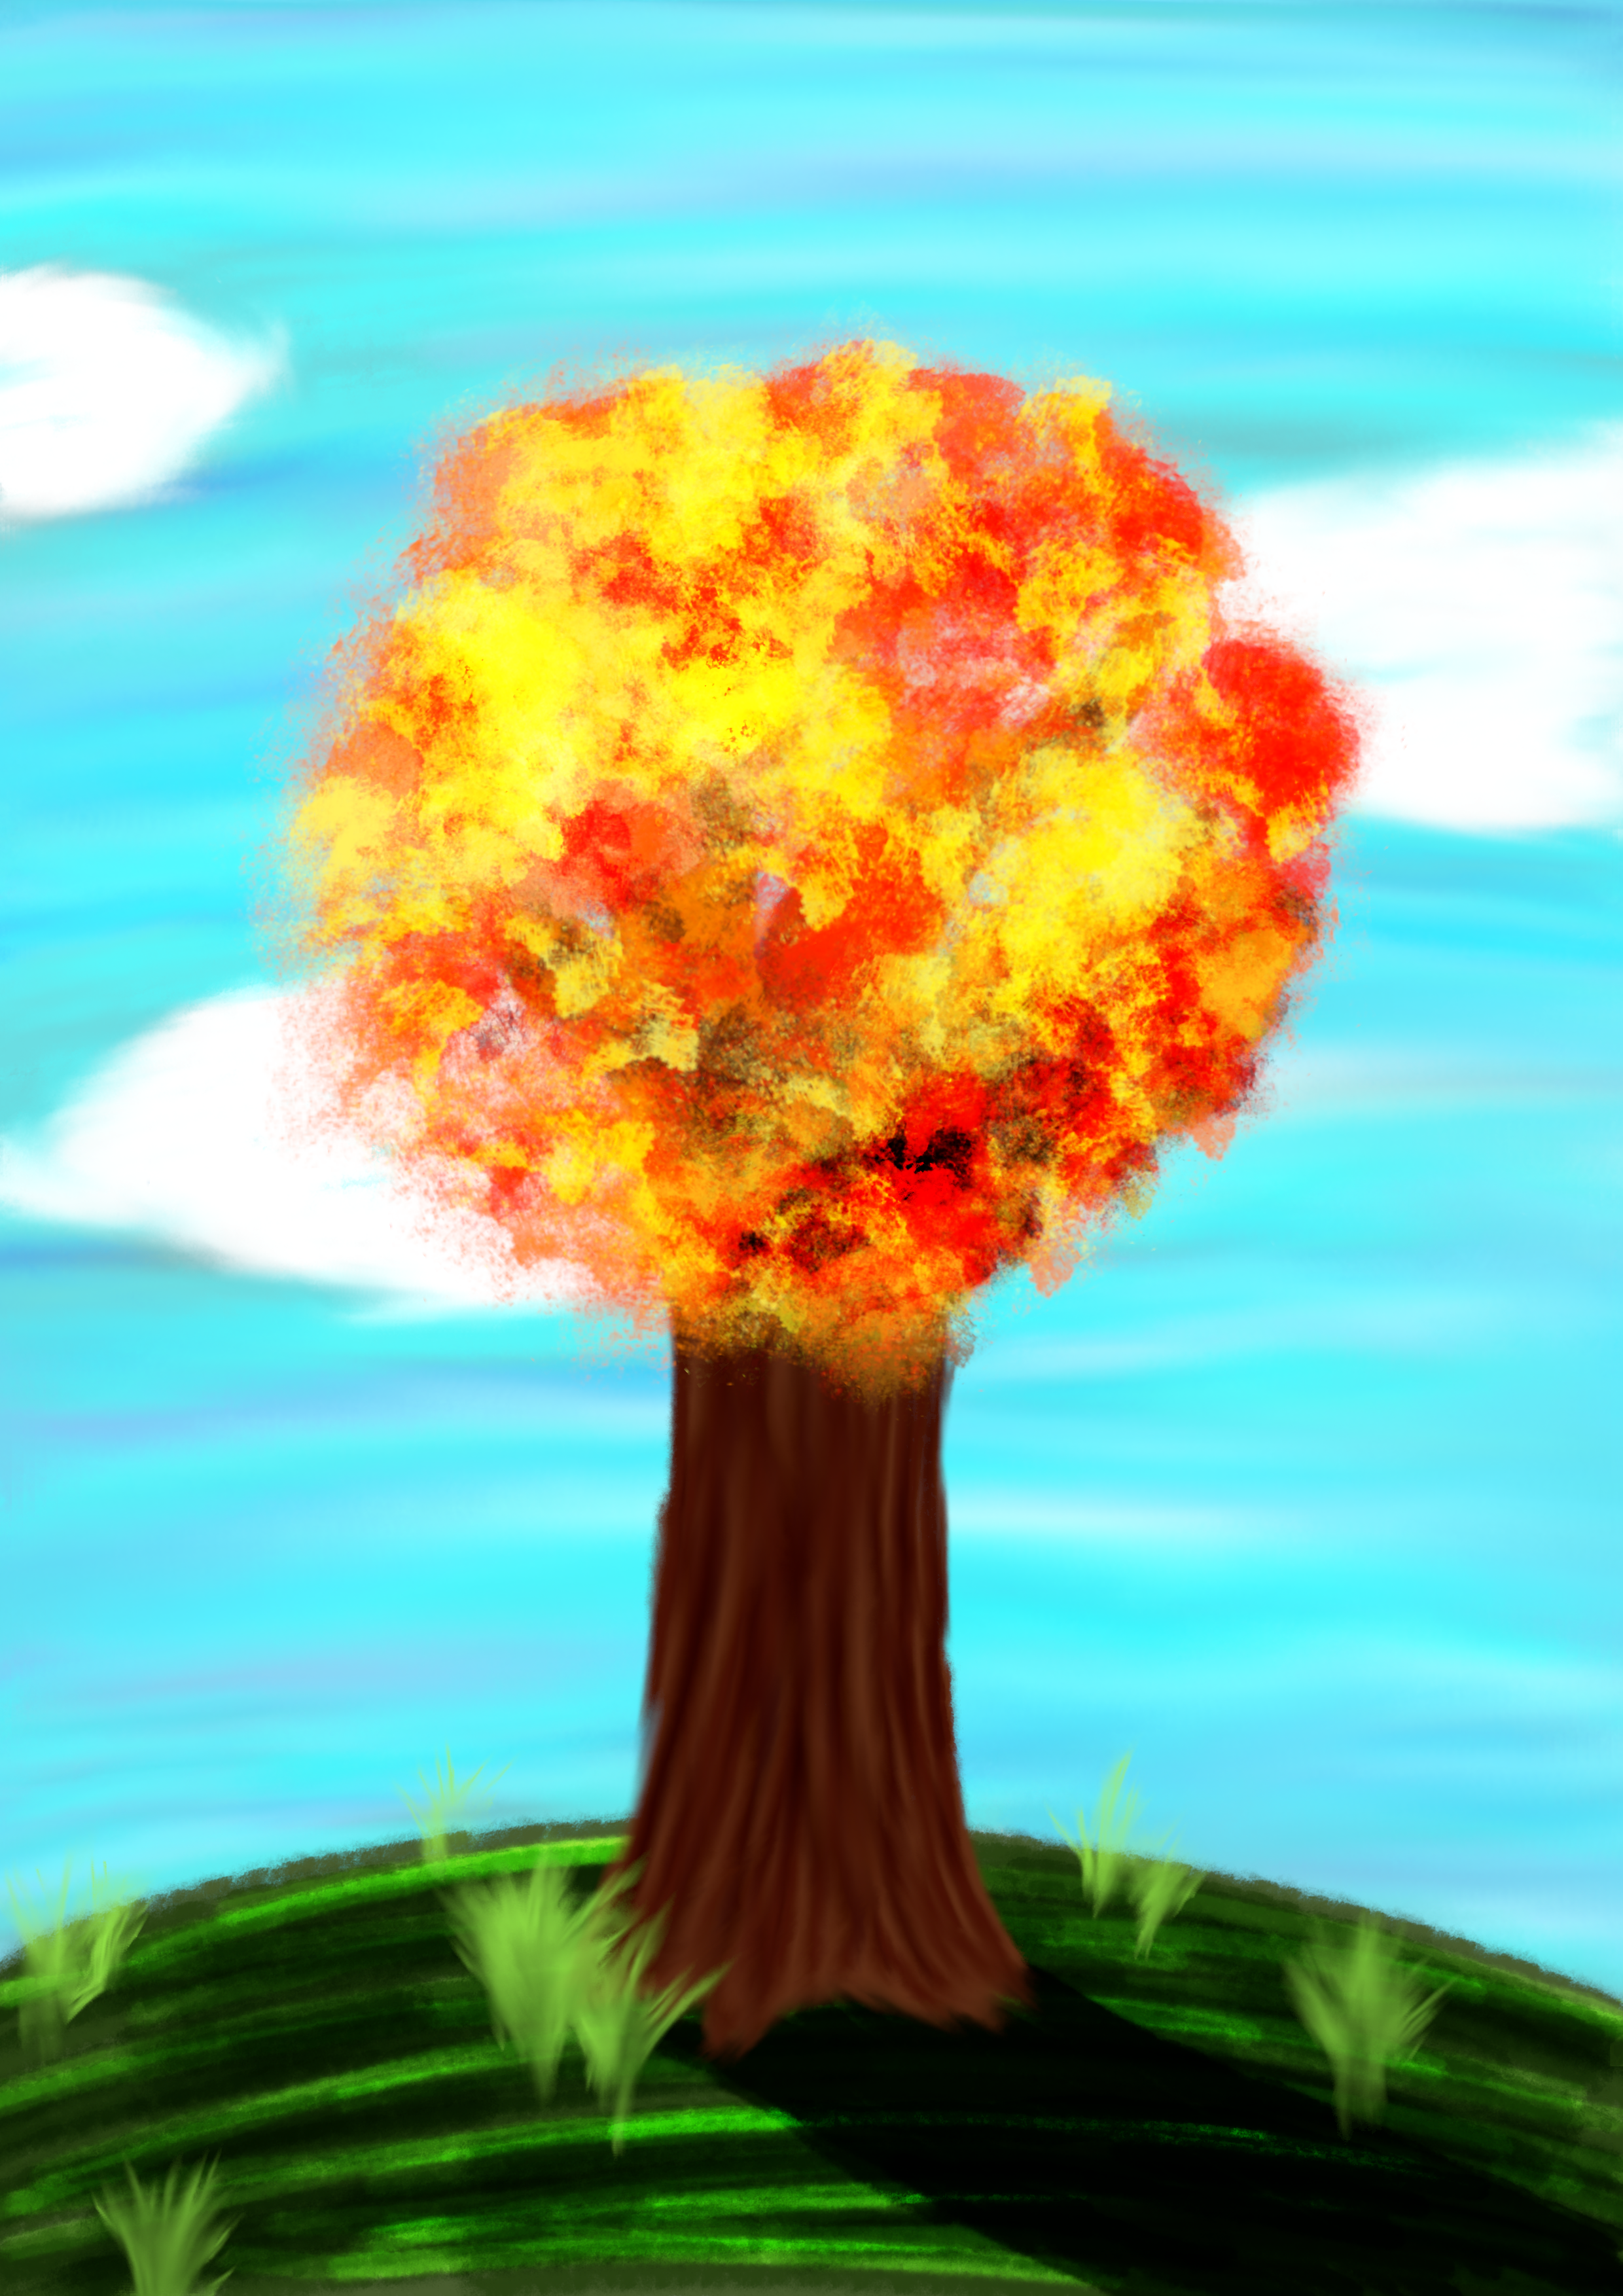
\includegraphics[height=0.4\textwidth]{logos/arbre.png}
    \end{minipage}
    \hfill
    \begin{minipage}[b]{0.3\textwidth}
      \centering
      James Bond\\
      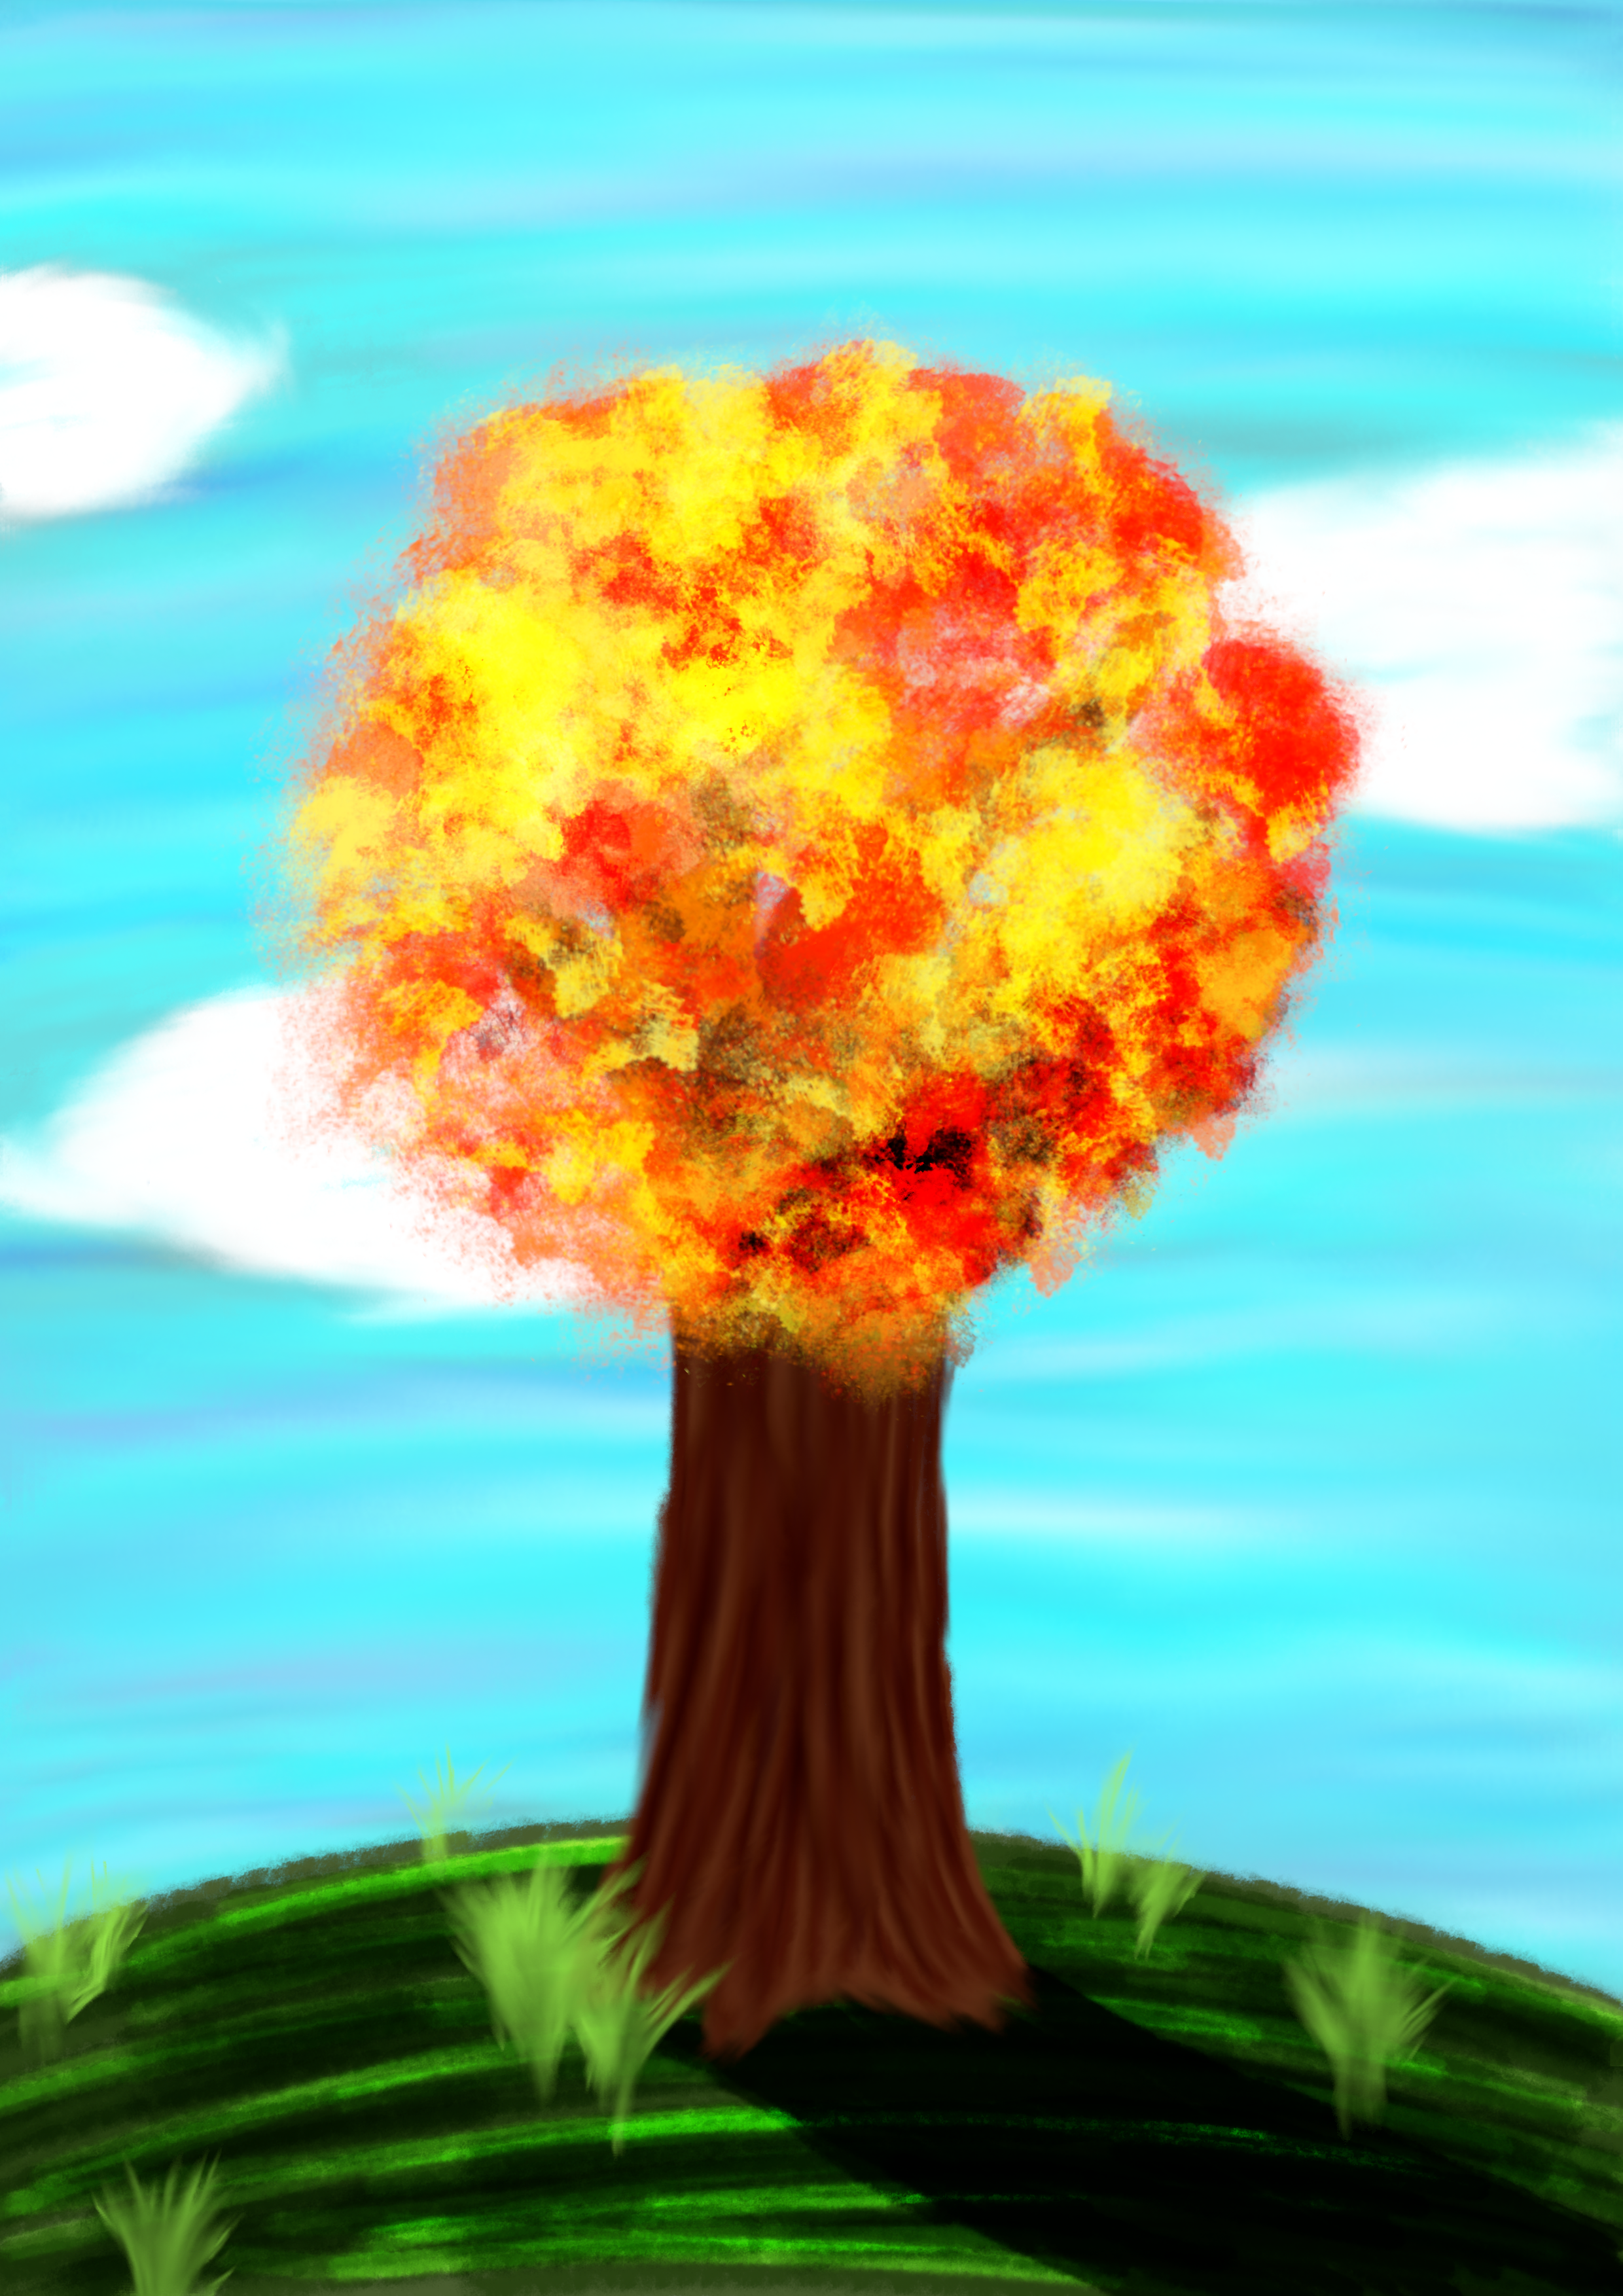
\includegraphics[height=0.4\textwidth]{logos/arbre.png}
    \end{minipage}
  \end{figure}

\newpage
\printbibliography % To generate the bibliography

\newpage
\appendix

% \includepdf[pages=1,pagecommand={\thispagestyle{empty}\vspace*{-3.3cm}\section{SKF 618/4}\label{pdf:skf 618_4}}]{PDF/Louis/618_4 SKF.pdf}
% \includepdf[pages=2-4]{PDF/Louis/618_4 SKF.pdf}




\end{document}
